\documentclass[aspectratio=169, 10pt]{beamer}

% Formal IEEE-style presentation theme with beautiful rounded shadows
\usetheme{Boadilla}
\usecolortheme{seahorse}
\usefonttheme{professionalfonts}

\usepackage{graphicx}
\usepackage{booktabs}
\usepackage{multirow}
\usepackage{tikz} 
\usepackage{pifont} % Added for checkmarks and crosses

% Enhancing visual appeal of lists and blocks
\setbeamertemplate{navigation symbols}{}
\setbeamertemplate{itemize item}{\color{blue!70!black}$\blacktriangleright$} 
\setbeamertemplate{itemize subitem}{\color{teal}$\bullet$}
\setbeamertemplate{caption}[numbered]
\setbeamertemplate{bibliography item}[text]
\setbeamertemplate{blocks}[rounded][shadow=true] 

% ==========================================
% HEADER LOGO CONFIGURATION
% ==========================================
% Added \IfFileExists to prevent compilation failures if image is missing in the environment
\addtobeamertemplate{frametitle}{}{%
\begin{tikzpicture}[remember picture,overlay]
\node[anchor=north east, yshift=-0.1cm, xshift=-0.2cm] at (current page.north east) {%
    \IfFileExists{faculty_of_engineering.jpeg}{
\includegraphics[height=1.5cm]{faculty_of_engineering.jpeg}}{}%
};
\end{tikzpicture}}

% ==========================================
% BULLETPROOF CUSTOM FOOTER
% ==========================================
\makeatletter
\setbeamertemplate{footline}{
  \leavevmode%
  \hbox{%
  \begin{beamercolorbox}[wd=.33\paperwidth,ht=2.5ex,dp=1.125ex,center]{author in head/foot}%
    \usebeamerfont{author in head/foot}\textbf{\insertshortauthor}
  \end{beamercolorbox}%
  \begin{beamercolorbox}[wd=.38\paperwidth,ht=2.5ex,dp=1.125ex,center]{title in head/foot}%
    \usebeamerfont{title in head/foot}\textbf{Reference-Guided Few-Shot Segmentation with Foundation Models , 2026}
  \end{beamercolorbox}%
  \begin{beamercolorbox}[wd=.29\paperwidth,ht=2.5ex,dp=1.125ex,right]{date in head/foot}%
    \usebeamerfont{date in head/foot}\textbf{Page \insertframenumber{} of \inserttotalframenumber}\hspace*{2ex}
  \end{beamercolorbox}}%
  \vskip0pt%
}
\makeatother

\title[Few-Shot Image Segmentation]{Reference-Guided Few-Shot Segmentation with Foundation Models}
%\subtitle{PhD Research Proposal}
\author[Omar Ahmed Fouad Hassan Wasfy]{Omar Ahmed Fouad Hassan Wasfy}
\institute[Alexandria University]{
Computer and Systems Engineering Department, Faculty of Engineering\\
 Alexandria University \\
 \vspace{1cm}
 \textbf{Supervisors: Prof. Dr. Mohamed Ismail and Prof. Dr. Nagia Ghanem}
 \\
 \vspace{0.5cm}
 \textbf{2026}
}
\date{} 

\begin{document}

% Slide 1
\begin{frame}
    \titlepage
\end{frame}

% Slide 2
\begin{frame}{Outline}
 \tableofcontents[hideallsubsections]
\end{frame}


% ==========================================
% SECTION 1: INTRODUCTION & BACKGROUND
% ==========================================
\section{Introduction \& Background}


% Slide X
\begin{frame}{Top-Tier Venues Referenced in This Presentation}

\begin{columns}[T]
    \begin{column}{0.48\textwidth}
        \begin{block}{Computer Vision}
            \begin{itemize}
                \item \textbf{CVPR} \\ \small IEEE/CVF Conference on Computer Vision and Pattern Recognition
                \item \textbf{ICCV} \\ \small IEEE/CVF International Conference on Computer Vision
                \item \textbf{IJCV} \\ \small International Journal of Computer Vision
                \item \textbf{TPAMI} \\ \small IEEE Transactions on Pattern Analysis and Machine Intelligence
            \end{itemize}
        \end{block}
    \end{column}

    \begin{column}{0.48\textwidth}
        \begin{block}{Machine Learning / AI}
            \begin{itemize}
                \item \textbf{ICLR} \\ \small International Conference on Learning Representations
                \item \textbf{NeurIPS} \\ \small Conference on Neural Information Processing Systems
                \item \textbf{AAAI} \\ \small AAAI Conference on Artificial Intelligence\\
                \hspace{0.5cm}\scriptsize (Association for the Advancement of Artificial Intelligence)
            \end{itemize}
        \end{block}
    \end{column}
\end{columns}

\vspace{0.3cm}
\centering
\footnotesize The listed venues comprise top-tier (A*) conferences and high-impact journals in Computer Vision and Machine Learning.
\end{frame}

% Slide 3
\begin{frame}{From Closed-Set \& Zero-Shot to Few-Shot Segmentation}
    \begin{columns}[T]
        \begin{column}{0.32\textwidth}
            \begin{alertblock}{Closed-Set Segmentation}
                \begin{itemize}
                    \item Trained on a \textbf{fixed, predefined} label space.
                    \item Requires \textbf{large-scale pixel-level annotations}.
                    \item \textbf{Limited generalization} to unseen object classes.
                \end{itemize}
            \end{alertblock}
        \end{column}

        \begin{column}{0.32\textwidth}
            \begin{block}{Zero-Shot Segmentation}
                \begin{itemize}
                    \item Transfers knowledge via \textbf{semantic priors} (e.g., \textit{text prompts}).
                    \item Utilizes \textbf{geometric prompts} (e.g., points, boxes).
                    \item Requires \textbf{no task-specific annotations}.
                    \item \textbf{Weak spatial precision} (coarse masks).
                \end{itemize}
            \end{block}
        \end{column}
        
        \begin{column}{0.32\textwidth}
            \begin{exampleblock}{Few-Shot Segmentation}
                \begin{itemize}
                    \item Adapts using \textbf{few labeled examples} (1--5 images) \cite{shaban2017one}.
                    \item Learns \textbf{class-specific representations} from support data.
                    \item \textbf{Accurate pixel-level localization}.
                    \item \textbf{Middle Ground:} balances generalization and supervision.
                \end{itemize}
            \end{exampleblock}
        \end{column}
    \end{columns}
\end{frame}

% Slide 4
\begin{frame}{Vision Foundation Models \& Visual Prompting}
    \begin{columns}[T]
        \begin{column}{0.48\textwidth}
            \begin{block}{Self-Supervised Learning at Scale}
                \begin{itemize}
                    \item Models trained on unprecedented scales of unannotated images (e.g., DINOv2) \cite{oquab2023dinov2}.
                    \item Discards traditional convolutions for long-range multi-head self-attention.
                    \item Yields highly robust feature embeddings with dense, part-level semantic understanding.
                \end{itemize}
            \end{block}
        \end{column}
        
        \begin{column}{0.48\textwidth}
            \begin{exampleblock}{Visual Conditioning (Prompting)}
                \begin{itemize}
                    \item \textbf{The Paradigm Shift:} Appends learnable tokens to input features while keeping massive foundation backbone weights \textbf{strictly frozen}.
                    \item Preserves generalized representation capacity.
                    \item Minimizes the risk of overfitting during adaptation where data is scarce.
                \end{itemize}
            \end{exampleblock}
        \end{column}
    \end{columns}
\end{frame}

% ==========================================
% SECTION 2: PROBLEM FORMULATION
% ==========================================
\section{Problem Formulation}

% Slide 5
\begin{frame}{Reference-Guided Few-Shot Segmentation \& System Setup}
    \begin{block}{Task Definition: Open-Set Generalization}
        A conditional dense prediction task aiming to delineate a target object in a query image, guided strictly by a small set of annotated reference examples. It operates \textbf{class-agnostic}, relying entirely on visual patterns rather than predefined text labels.
    \end{block}

    \begin{columns}[T]
        \begin{column}{0.48\textwidth}
            \textbf{Inputs}
            \begin{itemize}
                \item \textbf{Support Set (Reference Set):} A few images pairing the target object with a pixel-level spatial mask.
                \item \textbf{Query Image (Target Image):} Unlabeled target environment containing complex scenes and novel conditions.
            \end{itemize}
        \end{column}
        \begin{column}{0.48\textwidth}
            \textbf{Outputs \& Optimization}
            \begin{itemize}
                \item \textbf{Output:} A continuous probability map thresholded into a discrete binary mask.
                \item \textbf{Optimization:} A weighted dual-objective combination of Binary Cross-Entropy Loss and structural Dice Loss.
            \end{itemize}
        \end{column}
    \end{columns}
\end{frame}

% Slide 6
\begin{frame}{Core Technical Challenges}
    Adapting generic foundation models to Few-Shot Segmentation introduces severe mathematical bottlenecks:
    
    \begin{alertblock}{The Adaptation Challenges}
        \begin{itemize}
            \item \textbf{Cross-Image Correspondence:} Establishing associations despite radical differences in camera viewpoint, object pose, and lighting.
            \item \textbf{Appearance Variability:} Handling massive intra-class variation, scale changes, elastic deformation, and partial occlusion.
            \item \textbf{Distractor Suppression:} Distinguishing the target from visually similar elements densely clustered in complex environments.
            \item \textbf{Prompt Sensitivity:} Ensuring stability when automatically generated geometric prompts are placed suboptimally on object boundaries.
        \end{itemize}
    \end{alertblock}
\end{frame}

% ==========================================
% SECTION 3: APPLICATIONS
% ==========================================
\section{Applications}

% Slide 7
\begin{frame}{Real-World Applications}
    Addressing these challenges enables adaptive perception in dynamic scenarios:
    
    \begin{columns}[T]
        \begin{column}{0.48\textwidth}
            \begin{block}{Healthcare \& Robotics}
                \begin{itemize}
                    \item \textbf{Medical Image Analysis:} Segmenting rare structures or novel pathologies using highly limited annotated cases.
                    \item \textbf{Autonomous Manipulation:} Allowing robots to interact with previously unseen objects via human demonstration.
                \end{itemize}
            \end{block}
        \end{column}
        
        \begin{column}{0.48\textwidth}
            \begin{block}{Transport, Media \& AR}
                \begin{itemize}
                    \item \textbf{Autonomous Driving:} Segmenting unexpected road hazards or rare debris.
                    \item \textbf{Visual Search:} Locating specific instances in massive unstructured databases.
                    \item \textbf{Video Tracking:} Tracking a specific object across frames using a single anchor reference.
                \end{itemize}
            \end{block}
        \end{column}
    \end{columns}
\end{frame}

% ==========================================
% SECTION 4: FOUNDATION MODELS & SAM
% ==========================================
\section{Foundation Models \& SAM}

% Slide 8
\begin{frame}{The Segment Anything Model (SAM) \textbf{(ICCV 2023)}}
    % Top Section: Technical Description
    \begin{block}{Architecture \cite{kirillov2023segment}}
        \begin{itemize}
            \item \textbf{Image Encoder:} Masked Autoeconder (MAE) pre-trained Vision Transformer (ViT) generating high-dimensional image embeddings.
            \item \textbf{Prompt Encoder:} Positional encodings for points/boxes and convolutional layers for dense masks.
            \item \textbf{Mask Decoder:} Lightweight transformer mapping image and prompt embeddings to valid segmentation masks.
        \end{itemize}
    \end{block}

    \vfill % Adjusts vertical distribution

    % Bottom Section: Full-Width Visualization
    \centering
    \IfFileExists{SAM.png}{
        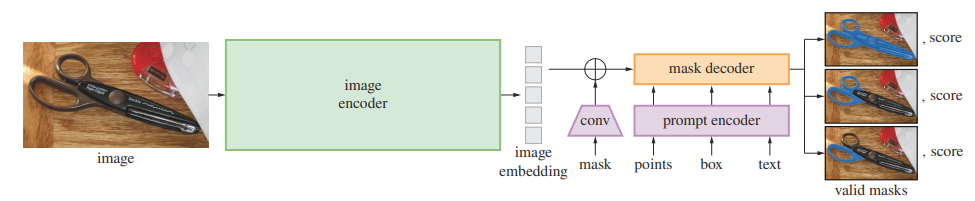
\includegraphics[width=\textwidth, height=0.45\textheight, keepaspectratio]{SAM.png}
    }{
        \begin{tikzpicture}
            \draw[dashed] (0,0) rectangle (\textwidth, 3) node[pos=.5] {Placeholder: SAM.png (Full Width)};
        \end{tikzpicture}
    }
\end{frame}

% Slide 10
\begin{frame}{The Semantic-Geometric Gap}
    \begin{block}{The Limitation of Scale (SA-1B Dataset)}
        SAM is trained on 1 billion high-quality masks, enforcing extreme geometric robustness. However, these masks are purely structural; they contain \textbf{no class or category labels}.
    \end{block}

    \begin{alertblock}{The Semantic Deficit}
        \begin{itemize}
            \item SAM learns \textit{"what constitutes an object"} but never learns \textit{"what the object is"}.
            \item It cannot natively process a support image-mask pair to locate a semantically identical object in a query image.
            \item External conditioning mechanisms must be engineered to translate semantic intent into SAM's native geometric prompt language.
        \end{itemize}
    \end{alertblock}
\end{frame}


% Slide 9: Qualitative Results
\begin{frame}{SAM Manual Prompting vs. Reference-Guided Segmentation}
    \begin{figure}[h]
        \centering
        \IfFileExists{VRP-SAM-1.png}{
            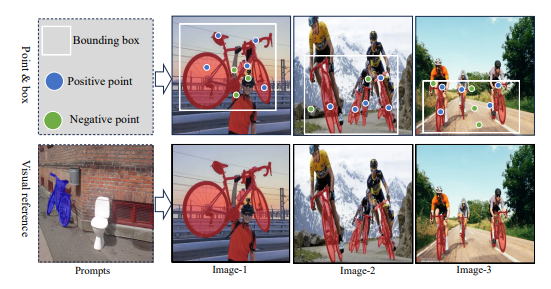
\includegraphics[width=\textwidth, height=0.85\textheight, keepaspectratio]{VRP-SAM-1.png}
        }{
            \begin{tikzpicture}
                \draw[dashed] (0,0) rectangle (\textwidth, 4) node[pos=.5] {Placeholder: VRP-SAM-1.png (Full Width)};
            \end{tikzpicture}
        }
    \end{figure}
\end{frame}


% ==========================================
% SECTION 5: ENHANCED METHODOLOGIES
% ==========================================
\section{Methodological Taxonomies}

% Slide 10

\begin{frame}{Taxonomy of SAM-based Adaptation Strategies}
    \begin{table}[htbp]
    \centering
    \caption{Classification of Representative Few-Shot SAM Adaptation Methods}
    \renewcommand{\arraystretch}{1.3}
    \small
    \begin{tabular}{l p{0.6\linewidth}}
    \toprule
    \textbf{Paper} & \textbf{Adaptation Strategy} \\
    \midrule
    VRP-SAM (CVPR 2024) \cite{sun2024vrp} & Prompt-based adaptation \\
    ProSAM (ICCV 2025) \cite{wang2025prosam} & Prompt-based adaptation (probabilistic prompting) \\
    Matcher (IJCV 2025 / ICLR 2024) \cite{liu2023matcher} & Feature matching-based adaptation \\
    DC-SAM (TPAMI 2025) \cite{qi2025dcsam} & Consistency-based adaptation \\
    Bridge the Points (NeurIPS 2024) \cite{zhang2024bridge} & Graph-based reasoning \\
    FCP-SAM (AAAI 2025) \cite{park2025fcpsam} & Prototype-based modeling \\
    \bottomrule
    \end{tabular}
    \end{table}
\end{frame}



% --- VRP-SAM ---
% Slide 11
\begin{frame}{VRP-SAM: Prompt-Based Adaptation \textbf{(CVPR 2024)}}
\textit{VRP-SAM: SAM with visual reference prompt.}
    \begin{columns}[T]
        \begin{column}{0.48\textwidth}
            \begin{block}{Motivation \& Concept \cite{sun2024vrp}}
                SAM relies on manual prompts. VRP-SAM automates this by extracting features via an auxiliary semantic encoder (ResNet) and generating compatible point embeddings via multi-head cross-attention.
            \end{block}
        \end{column}
        
        \begin{column}{0.48\textwidth}
            \begin{exampleblock}{Strengths}
                \begin{itemize}
                    \item[\textcolor{green!70!black}{\ding{51}}] Highly efficient baseline for real-time video applications.
                    \item[\textcolor{green!70!black}{\ding{51}}] Perfectly preserves SAM's native geometric boundary precision.
                \end{itemize}
            \end{exampleblock}
            \begin{alertblock}{Limitations}
                \begin{itemize}
                    \item[\textcolor{red}{\ding{55}}] Highly susceptible to prompt sensitivity.
                    \item[\textcolor{red}{\ding{55}}] Rigid prompts fail if the target undergoes severe structural deformation.
                \end{itemize}
            \end{alertblock}
        \end{column}
    \end{columns}
\end{frame}

% Slide 12
\begin{frame}{VRP-SAM: Architecture \textbf{(CVPR 2024)}}
    \begin{center}
        \IfFileExists{VRP-SAM-3.png}{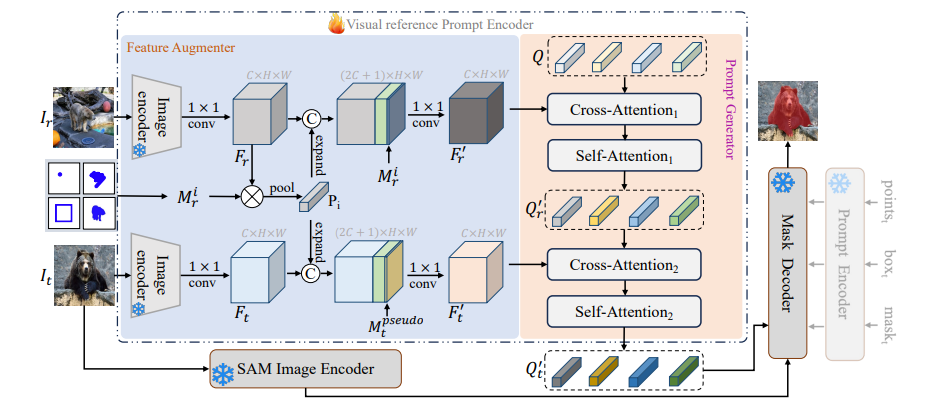
\includegraphics[width=\textwidth, height=0.85\textheight, keepaspectratio]{VRP-SAM-3.png}}{\textbf{[Placeholder: VRP-SAM-3.png]}}
    \end{center}
\end{frame}

% --- PROSAM ---
% Slide 13
\begin{frame}{ProSAM: Probabilistic Prompting \textbf{(ICCV 2025)}}
\textit{ProSAM: Enhancing the robustness of SAM-based visual reference segmentation with probabilistic prompts.}
    \begin{columns}[T]
        \begin{column}{0.48\textwidth}
            \begin{block}{Motivation \& Concept \cite{wang2025prosam}}
                Deterministic prompts are brittle. ProSAM models the prompt space as a continuous multivariate distribution. A Laplacian penalty physically pushes expected prompts toward flat, central regions of the target.
            \end{block}
        \end{column}
        
        \begin{column}{0.48\textwidth}
            \begin{exampleblock}{Strengths}
                \begin{itemize}
                    \item[\textcolor{green!70!black}{\ding{51}}] Exceptionally robust to boundary ambiguities.
                    \item[\textcolor{green!70!black}{\ding{51}}] Marginalizes uncertainty via Monte Carlo sampling.
                \end{itemize}
            \end{exampleblock}
            \begin{alertblock}{Limitations}
                \begin{itemize}
                    \item[\textcolor{red}{\ding{55}}] Processing multiple sampled prompts sequentially massively increases latency.
                    \item[\textcolor{red}{\ding{55}}] Unsuitable for high-speed tracking.
                \end{itemize}
            \end{alertblock}
        \end{column}
    \end{columns}
\end{frame}

% Slide 14
\begin{frame}{ProSAM: Architecture \textbf{(ICCV 2025)}}
    \begin{center}
        \IfFileExists{PRO-SAM-3.png}{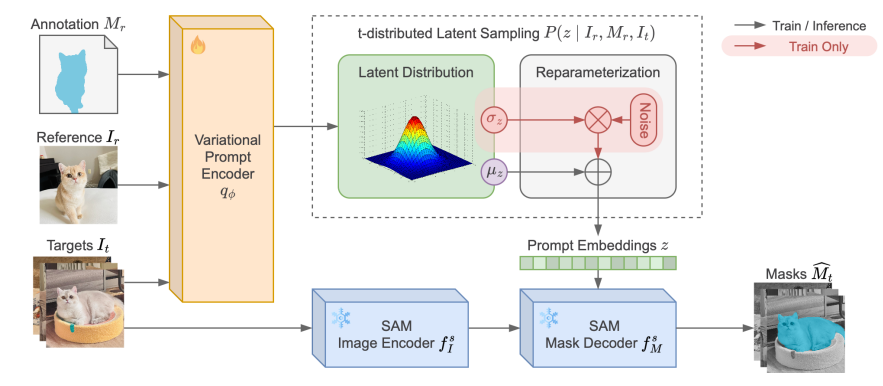
\includegraphics[width=\textwidth, height=0.85\textheight, keepaspectratio]{PRO-SAM-3.png}}{\textbf{[Placeholder: PRO-SAM-3.png]}}
    \end{center}
\end{frame}

% --- MATCHER ---
% Slide 15
\begin{frame}{Matcher: Feature Matching Approach \textbf{(IJCV 2025 \& ICLR 2024)}}
\textit{Matcher: Segment anything with one shot using all-purpose feature matching.}
    \begin{columns}[T]
        \begin{column}{0.48\textwidth}
            \begin{block}{Motivation \& Concept \cite{liu2023matcher}}
                Bypasses prompt training entirely. Constructs dense correlation volumes using DINOv2 self-supervised features and enforces forward/reverse cycle-consistency to eliminate mathematical outliers.
            \end{block}
        \end{column}
        
        \begin{column}{0.48\textwidth}
            \begin{exampleblock}{Strengths}
                \begin{itemize}
                    \item[\textcolor{green!70!black}{\ding{51}}] Elegant, tuning-free zero-shot operation.
                    \item[\textcolor{green!70!black}{\ding{51}}] Requires absolutely zero task-specific meta-training.
                \end{itemize}
            \end{exampleblock}
            \begin{alertblock}{Limitations}
                \begin{itemize}
                    \item[\textcolor{red}{\ding{55}}] Highly prone to distractor suppression failures. 
                    \item[\textcolor{red}{\ding{55}}] Visually similar background elements inevitably trigger false-positive matches.
                \end{itemize}
            \end{alertblock}
        \end{column}
    \end{columns}
\end{frame}

% Slide 16
\begin{frame}{Matcher: Architecture \textbf{(IJCV 2025 \& ICLR 2024)}}
    \begin{center}
        \IfFileExists{MATCHER-2.png}{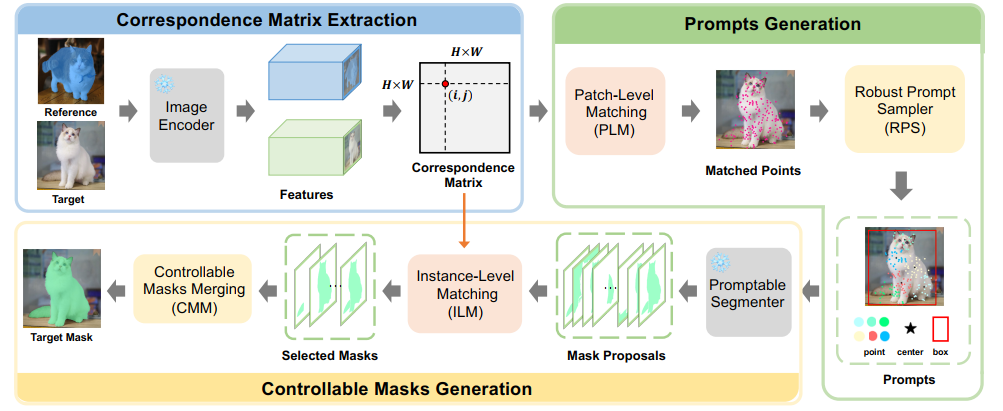
\includegraphics[width=\textwidth, height=0.85\textheight, keepaspectratio]{MATCHER-2.png}}{\textbf{[Placeholder: MATCHER-2.png]}}
    \end{center}
\end{frame}

% --- DC-SAM ---
% Slide 17
\begin{frame}{DC-SAM: Consistency-Based Adaptation \textbf{(TPAMI 2025)}}
\textit{DC-SAM: In-context segment anything in images and videos via dual consistency.}
    \begin{columns}[T]
        \begin{column}{0.48\textwidth}
            \begin{block}{Motivation \& Concept \cite{qi2025dcsam}}
                Addresses semantic drift onto adjacent objects. Maps initial coarse predictions back into prompt space to calculate deviation. Critically utilizes the inverted background mask as \textbf{explicit negative targets}.
            \end{block}
        \end{column}
        
        \begin{column}{0.48\textwidth}
            \begin{exampleblock}{Strengths}
                \begin{itemize}
                    \item[\textcolor{green!70!black}{\ding{51}}] Resolves semantic drift via cyclical validation.
                    \item[\textcolor{green!70!black}{\ding{51}}] Exceptional distractor suppression in densely cluttered scenes.
                \end{itemize}
            \end{exampleblock}
            \begin{alertblock}{Limitations}
                \begin{itemize}
                    \item[\textcolor{red}{\ding{55}}] Recursive cyclic attention loops heavily inflate memory footprint.
                    \item[\textcolor{red}{\ding{55}}] Restricts mobile or edge device deployment.
                \end{itemize}
            \end{alertblock}
        \end{column}
    \end{columns}
\end{frame}

% Slide 18
\begin{frame}{DC-SAM: Architecture \textbf{(TPAMI 2025)}}
    \begin{center}
        \IfFileExists{DC-SAM-2.png}{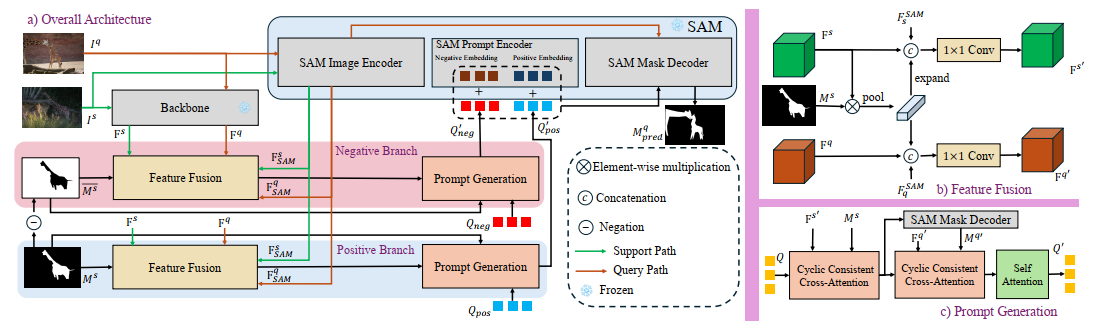
\includegraphics[width=\textwidth, height=0.85\textheight, keepaspectratio]{DC-SAM-2.png}}{\textbf{[Placeholder: DC-SAM-2.png]}}
    \end{center}
\end{frame}

% --- BRIDGE THE POINTS ---
% Slide 19
\begin{frame}{Bridge-the-Points: Graph-Based Reasoning \textbf{(NeurIPS 2024)}}

\textit{Bridge the points: Graph-based few-shot segment anything semantically.}

    \begin{columns}[T]
        \begin{column}{0.48\textwidth}
            \begin{block}{Motivation \& Concept \cite{zhang2024bridge}}
                Dense occlusion confuses standard pixel-wise attention. Maps spatial relationships as a directed graph. Clusters vertices by finding strongly connected components, isolating true targets from disconnected noise.
            \end{block}
        \end{column}
        
        \begin{column}{0.48\textwidth}
            \begin{exampleblock}{Strengths}
                \begin{itemize}
                    \item[\textcolor{green!70!black}{\ding{51}}] Manages severe occlusion without task-specific tuning.
                    \item[\textcolor{green!70!black}{\ding{51}}] Solves confusion from dense multi-instance co-occurrence.
                \end{itemize}
            \end{exampleblock}
            \begin{alertblock}{Limitations}
                \begin{itemize}
                    \item[\textcolor{red}{\ding{55}}] Graph traversal exhibits quadratic time complexity in worst case $\mathcal{O}(|\mathcal{V}|^2)$.
                    \item[\textcolor{red}{\ding{55}}] Introduces massive latency bottlenecks for high resolution images.
                \end{itemize}
            \end{alertblock}
        \end{column}
    \end{columns}
\end{frame}

% Slide 20
\begin{frame}{Bridge-the-Points: Architecture \textbf{(NeurIPS 2024)}}
    \begin{center}
        \IfFileExists{BRIDGE-THE-POINTS-1.png}{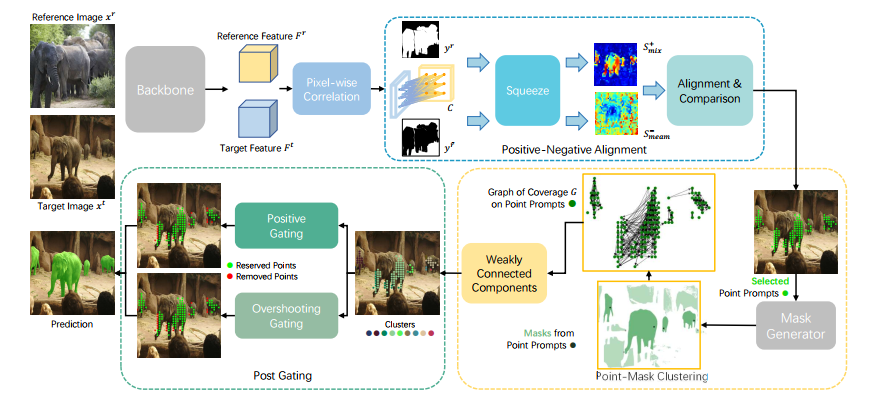
\includegraphics[width=\textwidth, height=0.85\textheight, keepaspectratio]{BRIDGE-THE-POINTS-1.png}}{\textbf{[Placeholder: BRIDGE-THE-POINTS-1.png]}}
    \end{center}
\end{frame}

% --- FCP-SAM ---
% Slide 21
\begin{frame}{FCP-SAM: Prototype-Based Modeling \textbf{(AAAI 2025)}}

\textit{Foreground-covering prototype generation and matching for SAM-aided few-shot segmentation.}
    \begin{columns}[T]
        \begin{column}{0.48\textwidth}
            \begin{block}{Motivation \& Concept \cite{park2025fcpsam}}
                Discrete points fail on non-rigid structures (e.g., netting). FCP-SAM abandons points, combining spatial granularity from SAM with class consistency from ResNet into a unified, dense prototype vector.
            \end{block}
        \end{column}
        
        \begin{column}{0.48\textwidth}
            \begin{exampleblock}{Strengths}
                \begin{itemize}
                    \item[\textcolor{green!70!black}{\ding{51}}] Exceptional global context modeling.
                    \item[\textcolor{green!70!black}{\ding{51}}] Highly stable multi-shot scaling (averaging dense prototypes).
                \end{itemize}
            \end{exampleblock}
            \begin{alertblock}{Limitations}
                \begin{itemize}
                    \item[\textcolor{red}{\ding{55}}] Heavy reliance on auxiliary backbones (ResNet).
                    \item[\textcolor{red}{\ding{55}}] Compromises the elegance of a pure foundation pipeline.
                \end{itemize}
            \end{alertblock}
        \end{column}
    \end{columns}
\end{frame}

% Slide 22
\begin{frame}{FCP-SAM: Architecture \textbf{(AAAI 2025)}}
    \begin{center}
        \IfFileExists{FCP-SAM-2.png}{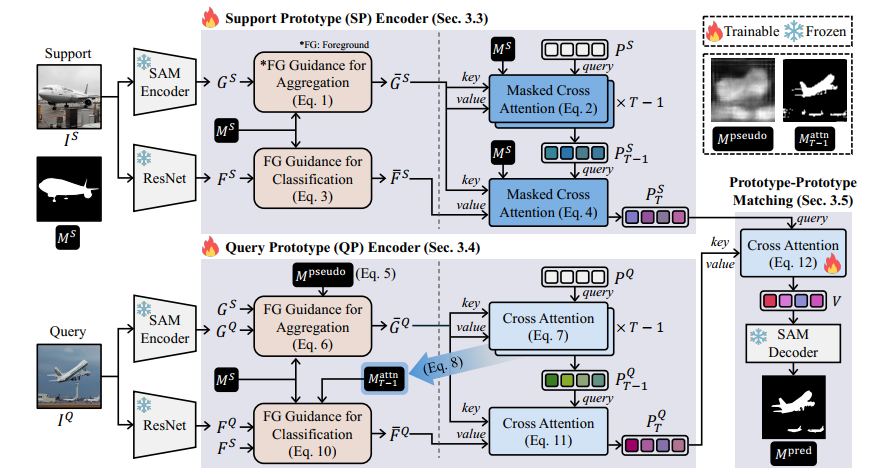
\includegraphics[width=\textwidth, height=0.80\textheight, keepaspectratio]{FCP-SAM-2.png}}{\textbf{[Placeholder: FCP-SAM-2.png]}}
    \end{center}
\end{frame}


% --- PerSAM ---
% Slide 17
\begin{frame}{PerSAM: Personalized One-Shot Adaptation \textbf{(ICLR 2024)}}
\textit{Personalize segment anything model with one shot.}
    \begin{columns}[T]
        \begin{column}{0.48\textwidth}
            \begin{block}{Motivation \& Concept \cite{zhang2024persam}}
                Standard SAM fails to segment specific user-designated instances. PerSAM establishes a target-guided attention mechanism via feature similarity and utilizes Parameter-Efficient Fine-Tuning (PEFT) to optimize only 2 scale-aware parameters.
            \end{block}
        \end{column}
        
        \begin{column}{0.48\textwidth}
            \begin{exampleblock}{Strengths}
                \begin{itemize}
                    \item[\textcolor{green!70!black}{\ding{51}}] Extremely lightweight adaptation (fine-tunes in $<$10 seconds).
                    \item[\textcolor{green!70!black}{\ding{51}}] High fidelity for specific instance tracking in videos.
                \end{itemize}
            \end{exampleblock}
            \begin{alertblock}{Limitations}
                \begin{itemize}
                    \item[\textcolor{red}{\ding{55}}] Performance drops under severe pose or lighting variations.
                    \item[\textcolor{red}{\ding{55}}] Reliant on high-quality initial feature matching.
                \end{itemize}
            \end{alertblock}
        \end{column}
    \end{columns}
\end{frame}

% --- DAPSAM ---
% Slide 18
\begin{frame}{DAPSAM: Domain-Adaptive Medical SDG \textbf{(MICCAI 2024)}}
\textit{Prompting SAM with domain-adaptive prototype for medical image segmentation.}
    \begin{columns}[T]
        \begin{column}{0.48\textwidth}
            \begin{block}{Motivation \& Concept \cite{wei2024prompting}}
                Bridges the natural-to-clinical domain gap (SDG). It injects domain-specific knowledge into SAM via learnable prototypes that handle low-contrast tissue boundaries and scanner variations in MRI/CT data.
            \end{block}
        \end{column}
        
        \begin{column}{0.48\textwidth}
            \begin{exampleblock}{Strengths}
                \begin{itemize}
                    \item[\textcolor{green!70!black}{\ding{51}}] Strong Single-Source Domain Generalization (SDG).
                    \item[\textcolor{green!70!black}{\ding{51}}] Effectively manages fuzzy anatomical boundaries.
                \end{itemize}
            \end{exampleblock}
            \begin{alertblock}{Limitations}
                \begin{itemize}
                    \item[\textcolor{red}{\ding{55}}] Requires representative clinical data for meta-training.
                    \item[\textcolor{red}{\ding{55}}] Added computational latency from domain-alignment modules.
                \end{itemize}
            \end{alertblock}
        \end{column}
    \end{columns}
\end{frame}





% ==========================================
% SECTION 6: COMPARATIVE STUDY & DISCUSSION
% ==========================================
\section{Comparative Study \& Discussion}

% Slide 24
\begin{frame}{Evaluation Datasets: Standard Baselines}
    \begin{block}{PASCAL-$5^i$ \cite{shaban2017one}}
        \begin{itemize}
            \item \textbf{Structure:} 20 object categories divided evenly across 4 test folds.
            \item \textbf{Visual Characteristics:} Images generally feature centered, single-dominant foreground objects with moderate occlusion.
            \item \textbf{Evaluation Role:} Serves as the foundational baseline entry-point for assessing basic foreground extraction precision.
        \end{itemize}
    \end{block}

    \begin{block}{MS COCO-$20^i$ \cite{nguyen2019feature}}
        \begin{itemize}
            \item \textbf{Structure:} 80 diverse categories split into 4 test folds.
            \item \textbf{Visual Characteristics:} Highly challenging scenes filled with dense multi-instance clutter, severe scale variation, and heavy subject occlusion.
            \item \textbf{Evaluation Role:} The primary "Distractor Challenge," rigorously testing the model's capacity to suppress visually similar background elements.
        \end{itemize}
    \end{block}
\end{frame}

% Slide 25
\begin{frame}{Evaluation Datasets: Large-Vocabulary Benchmarks}
    \begin{block}{FSS-1000 \cite{li2020fss}}
        \begin{itemize}
            \item \textbf{Structure:} 10,000 images spanning exactly 1,000 distinct, fine-grained categories.
            \item \textbf{Visual Characteristics:} Focuses on rare or unconventional objects against relatively clean backgrounds.
            \item \textbf{Evaluation Role:} Evaluates extreme open-set generalization on entities entirely absent from standard pre-training distributions.
        \end{itemize}
    \end{block}

    \begin{block}{LVIS-$92^i$ \cite{gupta2019lvis}}
        \begin{itemize}
            \item \textbf{Structure:} A severe long-tailed distribution exceeding 1,200 unique semantic categories.
            \item \textbf{Visual Characteristics:} Extremely rare entities embedded inside highly complex and varied spatial layouts.
            \item \textbf{Evaluation Role:} The ultimate scalability test, evaluating structural robustness against extreme data imbalance.
        \end{itemize}
    \end{block}
\end{frame}

% Slide 26
\begin{frame}{Evaluation Datasets: Part-Level Semantics}
    \begin{block}{PASCAL-Part \cite{chen2014detect}}
        \begin{itemize}
            \item \textbf{Structure:} High-resolution, fine-grained extension of the PASCAL VOC dataset.
            \item \textbf{Visual Characteristics:} Target regions frequently possess minimal visual contrast against adjacent sub-parts (e.g., separating a dog's leg from its torso).
            \item \textbf{Evaluation Role:} Validates the network's capacity for high-resolution, intra-object geometric localization.
        \end{itemize}
    \end{block}

    \begin{block}{PACO-Part \cite{ramanathan2023paco}}
        \begin{itemize}
            \item \textbf{Structure:} 75 distinct object categories, further subdivided into over 200 diverse part categories.
            \item \textbf{Visual Characteristics:} Features highly complex contextual interactions and ambiguous object-part compositions.
            \item \textbf{Evaluation Role:} Rigorous evaluation of fine-grained structural reasoning beyond coarse visual proxies.
        \end{itemize}
    \end{block}
\end{frame}

% Slide 27
\begin{frame}{Overall Results: Standard \& Large-Vocabulary Datasets}
    \vspace{-0.1cm}
    \begin{table}[htbp]
    \centering
    \caption{Overall Quantitative Results (mIoU \%)}
    \renewcommand{\arraystretch}{0.95} % Prevent vertical overflow
    \resizebox{\linewidth}{!}{
    \begin{tabular}{l l c c c c c c c c}
    \toprule
    \textbf{Method} & \textbf{Backbone} & \multicolumn{2}{c}{\textbf{PASCAL-5i}} & \multicolumn{2}{c}{\textbf{COCO-20i}} & \multicolumn{2}{c}{\textbf{FSS-1000}} & \multicolumn{2}{c}{\textbf{LVIS-92i}} \\
    \cmidrule(lr){3-4} \cmidrule(lr){5-6} \cmidrule(lr){7-8} \cmidrule(lr){9-10}
    & & \textbf{1-s} & \textbf{5-s} & \textbf{1-s} & \textbf{5-s} & \textbf{1-s} & \textbf{5-s} & \textbf{1-s} & \textbf{5-s} \\
    \midrule
    VRP-SAM \cite{sun2024vrp} & ResNet-50 & 71.9 & 72.9 & 53.9 & -- & -- & -- & -- & -- \\
    VRP-SAM \cite{sun2024vrp} & DINOv2 & -- & -- & 60.4 & -- & -- & -- & -- & -- \\
    ProSAM \cite{wang2025prosam} & ResNet-50 & 72.0 & -- & 54.6 & -- & -- & -- & -- & -- \\
    ProSAM \cite{wang2025prosam} & DINOv2 & -- & -- & 59.2 & -- & -- & -- & -- & -- \\
    Matcher \cite{liu2023matcher} & DINOv2 & -- & -- & 52.7 & 60.7 & 87.0 & \textbf{89.6} & 33.0 & 40.0 \\
    DC-SAM \cite{qi2025dcsam} & ResNet-50 & 73.0 & -- & 55.5 & -- & -- & -- & -- & -- \\
    DC-SAM \cite{qi2025dcsam} & DINOv2 & -- & -- & \textbf{62.0} & -- & -- & -- & -- & -- \\
    DC-SAM (SAM2) \cite{qi2025dcsam} & ResNet-50 & \textbf{74.0} & -- & 56.4 & -- & -- & -- & -- & -- \\
    Bridge-the-Points \cite{zhang2024bridge} & DINOv2 & 72.1 & \textbf{82.6} & 58.7 & \textbf{66.8} & \textbf{88.0} & 88.9 & \textbf{35.2} & \textbf{44.2} \\
    FCP-SAM \cite{park2025fcpsam} & ResNet-50 & 73.2 & 74.0 & 52.5 & 58.0 & -- & -- & -- & -- \\
    \bottomrule
    \multicolumn{10}{l}{\small \textit{}}
    \end{tabular}}
    \end{table}
\end{frame}

% Slide 28
\begin{frame}{Overall Results: Part-Level Semantics Datasets}
\vspace{-0.2cm}

\begin{table}[htbp]
\centering
\caption{Results (mIoU \%) on One-Shot Part Segmentation Datasets}
\renewcommand{\arraystretch}{1.2}
\small
\begin{tabular}{l c c}
\toprule
\textbf{Method} & \textbf{PASCAL-Part (1-shot)} & \textbf{PACO-Part (1-shot)} \\
\midrule
Matcher \cite{liu2023matcher} & 42.9 & 34.7 \\
Bridge-the-Points \cite{zhang2024bridge} & \textbf{44.5} & \textbf{36.3} \\
\bottomrule
\end{tabular}
\end{table}

\vspace{0.3cm}

\begin{alertblock}{Key Observation}
Part-level segmentation is significantly harder than whole-object segmentation.  
Graph-based reasoning (\textbf{Bridge-the-Points}) achieves the best performance by modeling structural relationships between object regions.
\end{alertblock}

\end{frame}

% Slide 29
\begin{frame}{Discussion I: Semantic Alignment \& Negative Prompting}
    \begin{alertblock}{The Necessity of Semantic Alignment}
        \begin{itemize}
            \item Empirical results decisively prove that SAM's native geometric prompts are computationally insufficient for dense open-set tasks.
            \item Pure geometric points cannot disambiguate visually similar regions without explicit prototype aggregation or cyclic semantic mapping.
        \end{itemize}
    \end{alertblock}

    \begin{exampleblock}{The Power of Negative Prompting}
        \begin{itemize}
            \item The most significant structural performance gains originate from explicitly treating non-target regions in the support image as \textbf{counterexamples}.
            \item Pushing target and background embeddings apart in the latent space is absolutely vital in highly cluttered datasets (COCO/LVIS).
        \end{itemize}
    \end{exampleblock}
\end{frame}




% Slide 30
\begin{frame}{Discussion II: Dataset Behavior \& Part-Level Challenges}
    \begin{block}{Dataset-Dependent Vulnerabilities}
        \begin{itemize}
            \item \textbf{Clean Scenes (PASCAL):} Lightweight prompt generators (VRP-SAM) remain highly competitive as simple geometry is sufficient.
            \item \textbf{Dense Clutter (COCO/LVIS):} Consistency enforcement (DC-SAM) and relational graphs (Bridge-the-Points) dominate by explicitly suppressing complex distractors.
        \end{itemize}
    \end{block}
    
    \begin{alertblock}{The Fine-Grained Semantic Challenge (PASCAL/PACO-Part)}
        \begin{itemize}
            \item Substantially lower absolute performance ($<45\%$ mIoU) confirms fine-grained intra-object reasoning remains a major bottleneck.
            \item Models heavily struggle to distinguish subtle boundaries where geometric contrast is minimal (e.g., a wheel attached to a frame).
        \end{itemize}
    \end{alertblock}
\end{frame}

% Slide 31
\begin{frame}{Discussion III: The Impact of Representation Quality}
    \begin{table}[htbp]
    \centering
    \caption{Impact of Backbone Choice on COCO-$20^i$ (1-Shot mIoU \%)}
    \resizebox{0.6\linewidth}{!}{
    \begin{tabular}{l c c c}
    \toprule
    \textbf{Method} & \textbf{ResNet-50} & \textbf{DINOv2} & \textbf{Absolute Gain} \\
    \midrule
    VRP-SAM \cite{sun2024vrp} & 53.90 & 60.40 & \textcolor{green!60!black}{\textbf{+6.50}} \\
    ProSAM \cite{wang2025prosam} & 54.63 & 59.16 & \textcolor{green!60!black}{\textbf{+4.53}} \\
    DC-SAM \cite{qi2025dcsam} & 55.50 & 62.00 & \textcolor{green!60!black}{\textbf{+6.50}} \\
    \bottomrule
    \end{tabular}}
    \end{table}

    \begin{exampleblock}{The Power of Self-Supervised Transformers}
        \begin{itemize}
            \item Replacing traditional CNNs (ResNet-50) with DINOv2 yields massive, consistent performance gains across all evaluated architectures.
            \item \textbf{Conclusion:} The foundation-model encoder mathematically dictates the ultimate performance ceiling by providing superior semantically aligned features.
        \end{itemize}
    \end{exampleblock}
\end{frame}


\begin{frame}{Discussion IV: Complexity Trade-Offs}
\begin{itemize}
\item \textbf{Real-Time Efficiency:} Lightweight, single-pass methods (\textcolor{teal}{VRP-SAM}) are fast but prone to fragmentation in complex scenes.

    \item \textbf{Intermediate Complexity:} Cross-image feature alignment (\textcolor{teal}{Matcher}) introduces additional cost due to dense support-query interactions.
    
    \item \textbf{Probabilistic Prompting:} Modeling prompt uncertainty (\textcolor{teal}{ProSAM}) improves robustness in ambiguous regions, at the cost of iterative sampling and increased inference time.
    
    \item \textbf{High Robustness, Higher Cost:} Multi-stage reasoning (\textcolor{teal}{DC-SAM, FCP-SAM}) improves robustness at the expense of increased memory and latency.
    
    \item \textbf{Graph Bottleneck:} Structural graph-based methods (\textcolor{teal}{Bridge-the-Points}) scale poorly with worst case $\mathcal{O}(|\mathcal{V}|^2)$ complexity.
\end{itemize}

\end{frame}

\begin{frame}{Discussion V: Systemic Limitations}
    \begin{alertblock}{Key Limitations}
        \begin{itemize}
            \item \textbf{Auxiliary Backbone Dependence:} Reliance on heavily parameterized networks (e.g., ResNet) increases computational burden and reduces architectural simplicity.
            
            \item \textbf{Annotation Sensitivity:} Performance degrades under noisy or imprecise support masks.
        \end{itemize}
    \end{alertblock}
\end{frame}

% ==========================================
% SECTION 7: RESEARCH GAPS & CONCLUSION
% ==========================================
\section{Research Gaps \& Conclusion}

% Slide 33
\begin{frame}{Research Gap I: The Multi-Shot Degradation Problem}
    \begin{alertblock}{The Failure of Naive Aggregation}
        \begin{itemize}
            \item Despite the intuitive expectation that more references equal better performance, $K$-shot settings ($K=5$) \textbf{do not} consistently outperform 1-shot configurations.
            \item If the target object exhibits severe pose, scale, or articulation changes across the 5 support examples, naive feature averaging mathematically dilutes discriminative cues.
        \end{itemize}
    \end{alertblock}
\end{frame}

% Slide 34
\begin{frame}{Research Gaps II: Scalability and Alignment}
    \begin{columns}[T]
        \begin{column}{0.48\textwidth}
            \begin{alertblock}{Scalability Constraints}
                \begin{itemize}
                    \item Methods achieving state-of-the-art accuracy rely on iterative cyclic refinement or massive graph traversal.
                    \item These strategies create severe latency bottlenecks, strictly prohibiting deployment in resource-constrained edge environments or high-FPS robotics.
                \end{itemize}
            \end{alertblock}
        \end{column}
        
        \begin{column}{0.48\textwidth}
            \begin{alertblock}{Representation Alignment}
                \begin{itemize}
                    \item Foundation models (SAM) lack inherent semantic correspondence between domains.
                    \item The current necessity of mapping support features via external, dense prototypes acts as a computational crutch rather than a fundamental solution.
                \end{itemize}
            \end{alertblock}
        \end{column}
    \end{columns}
\end{frame}

% Slide 35
\begin{frame}{Promising Future Directions}
    Future algorithmic development must focus on unifying strong semantic representations with highly efficient inference mechanisms:
    
    \begin{block}{Intrinsic Attention Integration}
        \begin{itemize}
            \item Bypassing slow, external auxiliary modules by injecting spatial prompts and \textbf{explicit negative constraints} directly into the Vision Transformer's native self-attention maps.
        \end{itemize}
    \end{block}
    
    \begin{block}{Parameter-Efficient Fine-Tuning (PEFT)}
        \begin{itemize}
            \item Fully freezing foundation models establishes a rigid upper performance bound.
            \item Selectively applying PEFT (e.g., LoRA, Visual Prompt Tuning) to the decoder allows gentle adaptation to reference tasks without inducing catastrophic forgetting of geometric priors.
        \end{itemize}
    \end{block}
\end{frame}

% Slide 36
\begin{frame}{Conclusion}
    \begin{exampleblock}{The Trajectory of Visual Perception}
        \begin{itemize}
            \item Reference-guided Few-Shot Segmentation (FSS) successfully integrates example-based task specification with the powerful, zero-shot geometric priors of massive foundation models.
            \item The inherent architectural rigidity in networks like SAM can be successfully circumvented via mathematically rigorous, multi-stage conditioning algorithms.
            \item Moving forward, robust open-world generalization will rely heavily on \textbf{topological structural awareness} and the explicit mathematical modeling of \textbf{negative background context}.
        \end{itemize}
    \end{exampleblock}
\end{frame}




% ==========================================
% REFERENCES
% ==========================================
\begin{frame}[allowframebreaks]{References}
    \bibliographystyle{IEEEtran}
    \begin{thebibliography}{10}

    \bibitem{kirillov2023segment}
    Kirillov, A., Mintun, E., Ravi, N., Mao, H., Rolland, C., Gustafson, L., ... \& Girshick, R. (2023). Segment anything. In \textit{Proceedings of the IEEE/CVF International Conference on Computer Vision} (pp. 4015-4026).

    \bibitem{he2016deep}
    He, K., Zhang, X., Ren, S., \& Sun, J. (2016). Deep residual learning for image recognition. In \textit{Proceedings of the IEEE conference on computer vision and pattern recognition} (pp. 770-778).

    \bibitem{oquab2023dinov2}
    Oquab, M., Darcet, T., Moutakanni, T., Vo, H., Szafraniec, M., Khalidov, V., ... \& Bojanowski, P. (2023). Dinov2: Learning robust visual features without supervision. \textit{arXiv preprint arXiv:2304.07193}.

    \bibitem{dosovitskiy2020image}
    Dosovitskiy, A., Beyer, L., Kolesnikov, A., Weissenborn, D., Zhai, X., Unterthiner, T., ... \& Houlsby, N. (2020). An image is worth 16x16 words: Transformers for image recognition at scale. \textit{International Conference on Learning Representations}.

    \bibitem{shaban2017one}
    Shaban, A., Bansal, S., Liu, Z., Essa, I., \& Boots, B. (2017). One-shot learning for semantic segmentation. In \textit{Proceedings of the British Machine Vision Conference (BMVC)}.

    \bibitem{nguyen2019feature}
    Nguyen, K., \& Todorovic, S. (2019). Feature weighting and boosting for few-shot segmentation. In \textit{Proceedings of the IEEE/CVF International Conference on Computer Vision} (pp. 622-631).

    \bibitem{everingham2010pascal}
    Everingham, M., Van Gool, L., Williams, C. K., Winn, J., \& Zisserman, A. (2010). The pascal visual object classes (voc) challenge. \textit{International journal of computer vision}, 88(2), 303-338.

    \bibitem{lin2014microsoft}
    Lin, T. Y., Maire, M., Belongie, S., Hays, J., Perona, P., Ramanan, D., ... \& Zitnick, C. L. (2014). Microsoft coco: Common objects in context. In \textit{European conference on computer vision} (pp. 740-755). Springer, Cham.

    \bibitem{li2020fss}
    Li, X., Wei, T., Chen, Y. P., Tai, Y.-W., \& Tang, C.-K. (2020). Fss-1000: A 1000-class dataset for few-shot segmentation. In \textit{Proceedings of the IEEE/CVF conference on computer vision and pattern recognition} (pp. 2869-2878).

    \bibitem{gupta2019lvis}
    Gupta, A., Dollar, P., \& Girshick, R. (2019). Lvis: A dataset for large vocabulary instance segmentation. In \textit{Proceedings of the IEEE/CVF conference on computer vision and pattern recognition} (pp. 5356-5364).

    \bibitem{chen2014detect}
    Chen, X., Mottaghi, R., Liu, X., Fidler, S., Urtasun, R., \& Yuille, A. (2014). Detect what you can: Detecting and representing objects using holistic models and body parts. In \textit{Proceedings of the IEEE conference on computer vision and pattern recognition} (pp. 1971-1978).

    \bibitem{ramanathan2023paco}
    Ramanathan, V., Kalia, A., Petrovic, V., Wen, Y., Zheng, B., Guo, B., ... \& Marquez, A. (2023). Paco: Parts and attributes of common objects. \textit{arXiv preprint arXiv:2301.01795}.

    \bibitem{wang2019panet}
    Wang, K., Liew, J. H., Zou, Y., Zhou, D., \& Feng, J. (2019). PANet: Few-shot image semantic segmentation with prototype alignment. In \textit{Proceedings of the IEEE/CVF International Conference on Computer Vision} (pp. 9197-9206).

    \bibitem{tian2020pfenet}
    Tian, Z., Zhao, H., Shu, M., Yang, Z., Li, R., \& Jia, J. (2020). Prior guided feature enrichment network for few-shot segmentation. \textit{IEEE Transactions on Pattern Analysis and Machine Intelligence}, 44(2), 1050-1065.

\bibitem{sun2024vrp}
Sun, Y., Chen, J., Zhang, S., Zhang, X., Chen, Q., Zhang, G., \& Li, Z. (2024).
VRP-SAM: SAM with visual reference prompt.
In \textit{Proceedings of the IEEE/CVF Conference on Computer Vision and Pattern Recognition (CVPR)} (pp. 23565--23574).

\bibitem{wang2025prosam}
Wang, X., Sebastian, C., He, W., \& Ren, L. (2025).
ProSAM: Enhancing the robustness of SAM-based visual reference segmentation with probabilistic prompts.
In \textit{Proceedings of the IEEE/CVF International Conference on Computer Vision (ICCV)} (pp. 20487--20496).

\bibitem{liu2023matcher}
Liu, Y., Zhu, M., Li, H., Chen, H., Wang, X., \& Shen, C. (2023).
Matcher: Segment anything with one shot using all-purpose feature matching.
\textit{arXiv preprint arXiv:2305.13310}.

\bibitem{qi2025dcsam}
Qi, M., Zhu, P., Li, X., Bi, X., Qi, L., Ma, H., \& Yang, M. H. (2025).
DC-SAM: In-context segment anything in images and videos via dual consistency.
\textit{IEEE Transactions on Pattern Analysis and Machine Intelligence}.

\bibitem{zhang2024bridge}
Zhang, A., Gao, G., Jiao, J., Liu, C., \& Wei, Y. (2024).
Bridge the points: Graph-based few-shot segment anything semantically.
In \textit{Advances in Neural Information Processing Systems (NeurIPS)}, 37, 33232--33261.

\bibitem{park2025fcpsam}
Park, S., Lee, S., Seong, H. S., Yoo, J., \& Heo, J. P. (2025).
Foreground-covering prototype generation and matching for SAM-aided few-shot segmentation.
In \textit{Proceedings of the AAAI Conference on Artificial Intelligence}, 39(6), 6425--6433.

    \end{thebibliography}
\end{frame}


% Slide 37 (Thank You Slide)
\begin{frame}
    \frametitle{Thank You}
    \vfill
    \centering
    
\includegraphics[width=1\linewidth,height=0.79\textheight,keepaspectratio]{thankyou.png}
    
    \begin{flushright}
        \tiny\textbf{Email: omar.wasfy@alexu.edu.eg}
    \end{flushright}
    \vfill
\end{frame}



\end{document}